\section{Method}

We started with identification of common patterns occurring in the sample sequences that we would use to test our eye tracker on. Based on these patterns we have then formed our ideas of how should the software perform the detection. The patterns we have observed are as follows:

\begin{enumerate}

\item All sequences are taken with an IR camera, therefore the image has low chromaticity, but high luminance response. Therefore color could not be used to detect the eye, only the intensity.
\item Similarly, all sequences have resolution of 640x480 pixels, as a result of being taken with a web cam.
\item In all sequences there is one and only one eye, even though blinks can occur, so no pupil is visible
\item All sequences are shorter than 30 seconds

\end{enumerate}

We have built our eye tracker with these assumptions, so if any of them is broken (apart from 4.), our software will probably struggle to give a correct result. Another consideration we have made is that the performance is not the objective at this stage, so we have preferred solutions that are correct and complete over solutions that are fast. That being said, the software could still be optimized for performance and lower memory footprint removing a lot of repetition of the same calculations and code that has been introduced to enable parametrization of our partial functions.

The following subsections detail the concrete methods we have applied to get pupil, iris and glints from the images. All of them work on grayscale images.

\subsection{Pupil Detection}
For pupil detection we start off by computing k-means for a downsized grayscale image. K-means algorithm iteratively partitions all the pixels into k clusters, where each pixel belongs to a cluster with the nearest mean. In praxis this means that it will separate different levels of gray into separate regions. You can see an example of k-means clustering on Figure \ref{fig:kmeans}.

\begin{figure}[h!]
\centering
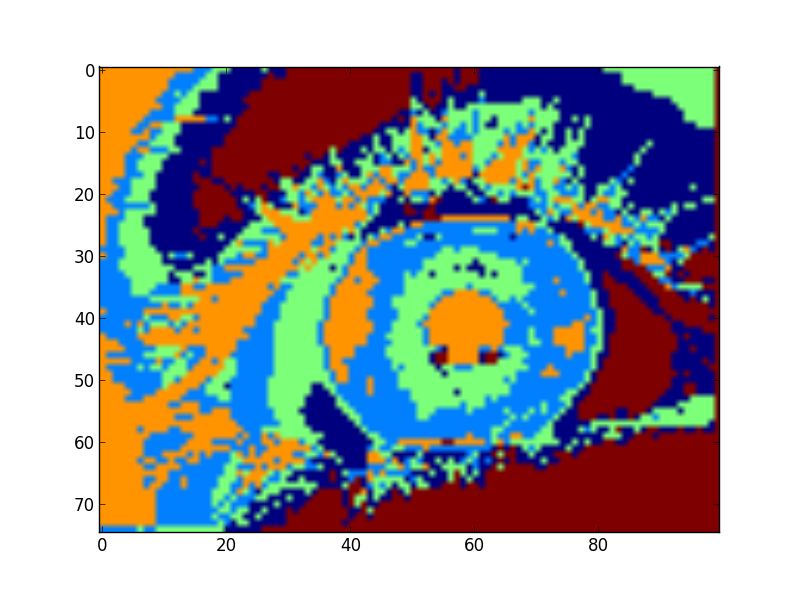
\includegraphics[width=\columnwidth]{Handin1/images/k-means.png}
\caption{k-means clustering}
\label{fig:kmeans}
\end{figure}

Since the pupil is usually very dark, it is (in most cases) safe to assume that it will be contained in the first cluster (the darkest). Therefore k-means can be used in this way to circumvent the need of setting threshold values for the thresholding function that comes next. Instead of a pre-chosen threshold we simply use the value of the first cluster. That ensures that the threshold will be set to contain the darkest values in the image (and by extension likely the pupil). The thresholded image obtained using the k-means from Figure \ref{fig:kmeans} can be seen in Figure \ref{subfig:thresh}. 

\begin{figure}[h!]
	\centering
	
	\begin{subfigure}[b]{0.5\textwidth}
		\centering
		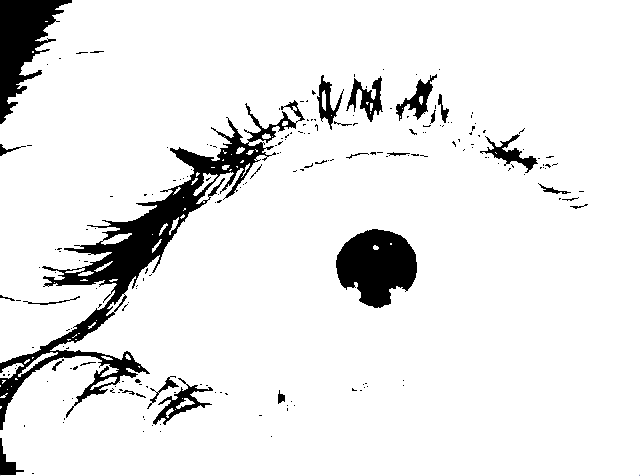
\includegraphics[width=\textwidth]{Handin1/images/thresh.png}
		\caption{After Thresholding}
		\label{subfig:thresh}
	\end{subfigure}%
	~
	\begin{subfigure}[b]{0.5\textwidth}
		\centering
		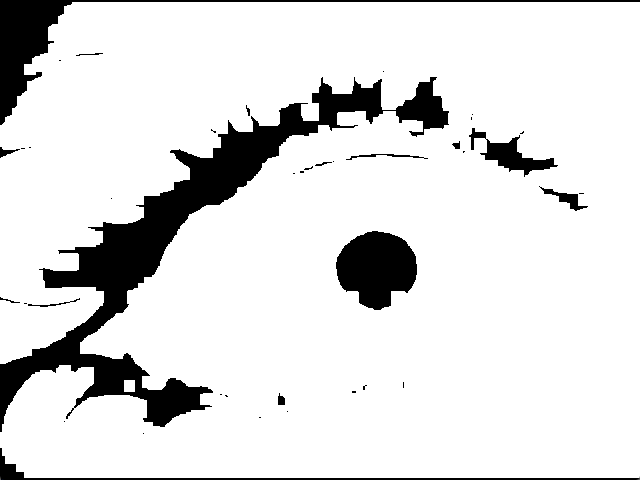
\includegraphics[width=\textwidth]{Handin1/images/open.png}
		\caption{After Opening}
		\label{subfig:open}
	\end{subfigure}
	
	\caption{Thresholding and Opening}
	\label{fig:threshopen}
\end{figure}

After thesholding we perform opening. Opening is a morphological operation that consists of performing erosion followed by dilation. This cleans up the image, removing noise and speckles. You can see this in the Figure \ref{subfig:open}



\subsection{Iris Detection}

\subsection{Glint Detection}